\documentclass[wide,a4paper,titlepage,12pt]{mwart}
\usepackage{polski,graphicx,pdflscape}
\usepackage[utf8]{inputenc}
\usepackage{listings}


\title{Filtr SOI}
\author{Tymon Tobolski (181037)\\ Jacek Wieczorek (181043)}

% Title page layout (fold)
\makeatletter
\renewcommand{\maketitle}{
\begin{titlepage}
  \begin{center}
    \vspace*{3cm}
    \LARGE \@title \par
    \vspace{2cm}
    \textit{\small Autor:}\par
    \normalsize \@author\par \normalsize
    \vspace{3cm}
    \textit{\small Prowadzący:}\par
    Dr inż. Paweł Biernacki \par
    \vspace{2cm}
    Wydział Elektroniki\\ II rok\\ WT/TN 13:15--15:00 \par
    \vspace{5cm}
    \small \@date
  \end{center}
\end{titlepage}
}
\makeatother
% Title page layout (end)

\begin{document}
  \maketitle
  \section{Cel ćwiczenia} % (fold)
  \label{sec:Cel}
    Badanie wpływu rzędu oraz okna filtru na jego charakterystyke.
    
  \section{Algorytm przetwarzający}
    Wykorzystane funkcje:
    \newline
    \begin{itemize}
      \item filtr (\textbf{fir1})
			\item charakterystyka (\textbf{freqz})
			\item okna (\textbf{hanning}, \textbf{hamming}, \textbf{gausswin}, \textbf{bartlett}, \textbf{kaiser})
    \end{itemize}
  
  \lstset{ %
    language=Octave,                % choose the language of the code
    basicstyle=\scriptsize,       % the size of the fonts that are used for the code
    numbers=left,                   % where to put the line-numbers
    numberstyle=\scriptsize,      % the size of the fonts that are used for the line-numbers
    stepnumber=10,                   % the step between two line-numbers. If it's 1 each line 
                                    % will be numbered
    numbersep=9pt,                  % how far the line-numbers are from the code
    % backgroundcolor=\color{white},  % choose the background color. You must add \usepackage{color}
    showspaces=false,               % show spaces adding particular underscores
    showstringspaces=false,         % underline spaces within strings
    showtabs=false,                 % show tabs within strings adding particular underscores
    % frame=single,                 % adds a frame around the code
    % tabsize=2,                  % sets default tabsize to 2 spaces
    % captionpos=b,                   % sets the caption-position to bottom
    breaklines=true,                % sets automatic line breaking
    % breakatwhitespace=false,        % sets if automatic breaks should only happen at whitespace
    % title=\lstname,                 % show the filename of files included with \lstinputlisting;
                                    % also try caption instead of title
    % escapeinside={\%*}{*)},         % if you want to add a comment within your code
    % morekeywords={*,...}            % if you want to add more keywords to the set
    }
    \lstinputlisting{lab5.m}
    
  % section Wstęp (end)
  
	\section{Wpływ rzędu filtru na jego charakterystyke częstotliwościową}
		Wraz ze wzrostem rzędu filtru SOI możemy zaobserwować, że krzywa oznaczająca pasmo przepustowości dąży do porstej pionowej. Dzieje się tak dlatego, że wraz ze wzrostem rzędu filtru maleje szerokośc pasma przejściowego, które dąży do coraz węższej wartości, co wpływa pozytywnie na ogólną ocene filtru..
		
		
		Zwiększenie wartości rzędu filtru SOI powoduje również zmianę wartości pasma zaporowego, odpowiadającego za zmniejszanie amplitudy sygnału. Zwiększa się szerokość pasma i dąży ono do uokresowienia się, co wpływa korzystnie na jakość filtru..
		
		
		Wraz z uokresowieniem pasma zaporowego, uokresowiony piłokształtnie zostaje wykres fazowy filtru. Dla pasma przepustowgo charakterystyka fazowa pozostaje liniowa. Jest to prawidłowe zachowanie filtru.
		
		Wykresy znajdują się na stronach \pageref{fig1}-\pageref{fig4}.
	
	\section{Wpływ rodzaju okna na charakterystyke częstotliwościową filtru}
	Wykres pasma przejściowego dla okna hamming, hanninga, gausswin oraz bartlett jest bardzo zbliżony. Różni sie głównie niewielkimi różnicami w poziomie zafalowań. Duża różnica w poziomie zafalowań widoczna jest w charakterystyce filtru z użyciem okna kaisera. Podobnie jest dla pasma zaporowego. Dla pierwszej grupy okien wykres różni się troche pofałdowaniem i połóżeniem zafalowań, natomista dla okna kaisera występuje ich znacznie więcej. Wykres fazowy zachowuje się podobnie jak w poprzednim podpunkcie dotyczącym badania rzędu filtru SOI.
	
	Wykresy znajdują się na stronach \pageref{fig5}-\pageref{fig9}.
	
		
	\begin{landscape}
	  \begin{figure}[htbp]
	    \begin{center}
	      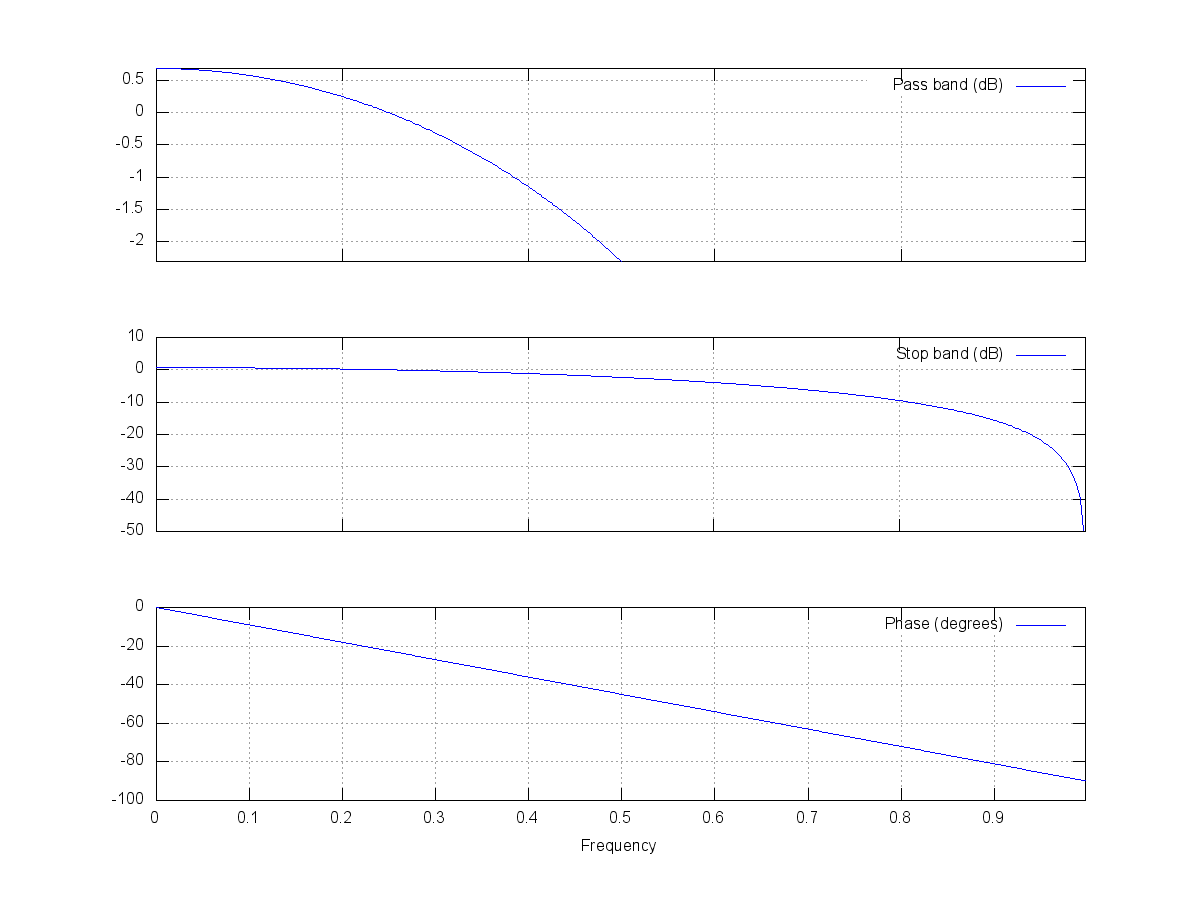
\includegraphics[scale=.5]{out/fig1.png}
	      \caption{\label{fig1} Rząd filtru: 1}
	    \end{center}
	  \end{figure}
	\end{landscape}
	
	\begin{landscape}
	  \begin{figure}[htbp]
	    \begin{center}
	      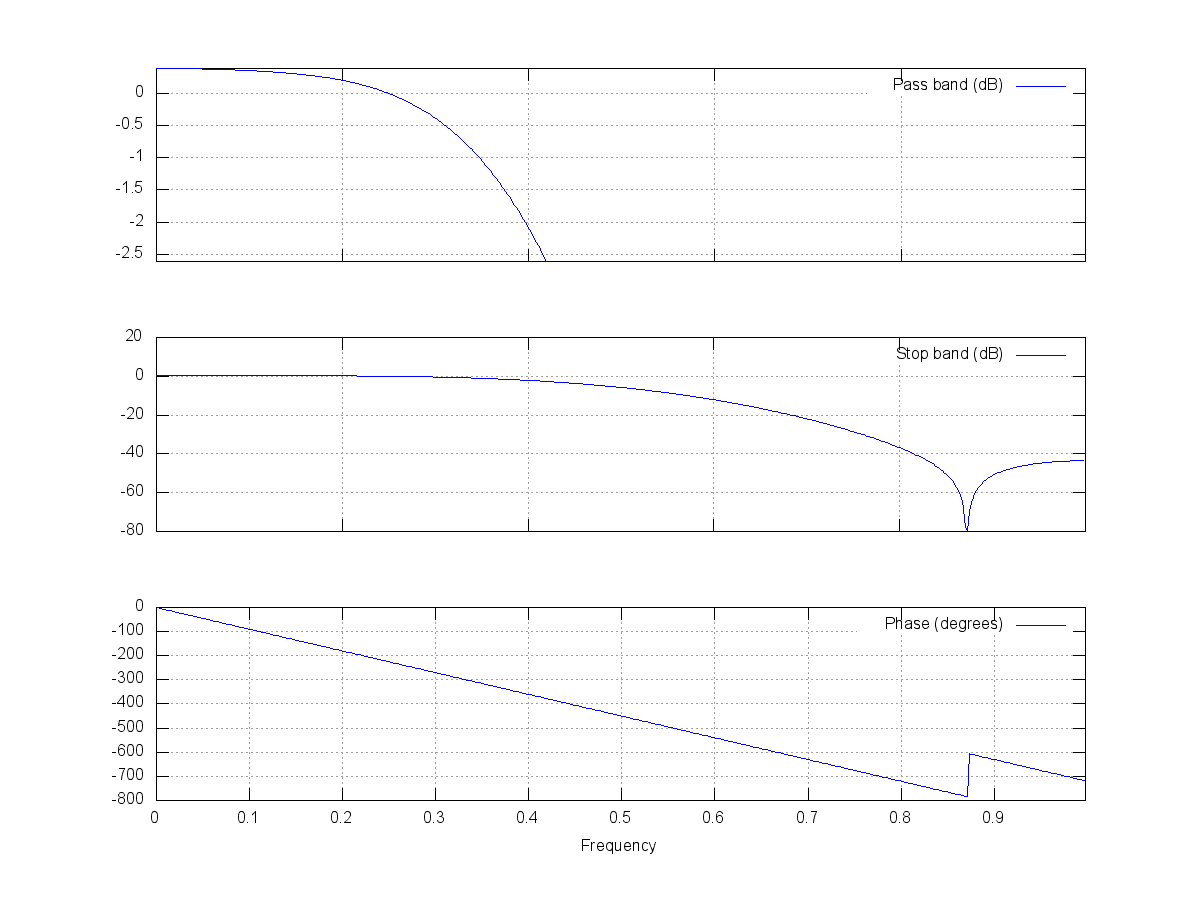
\includegraphics[scale=.5]{out/fig2.png}
	      \caption{\label{fig2}  Rząd filtru: 10}
	    \end{center}
	  \end{figure}
	\end{landscape}
	
	\begin{landscape}
	  \begin{figure}[htbp]
	    \begin{center}
	      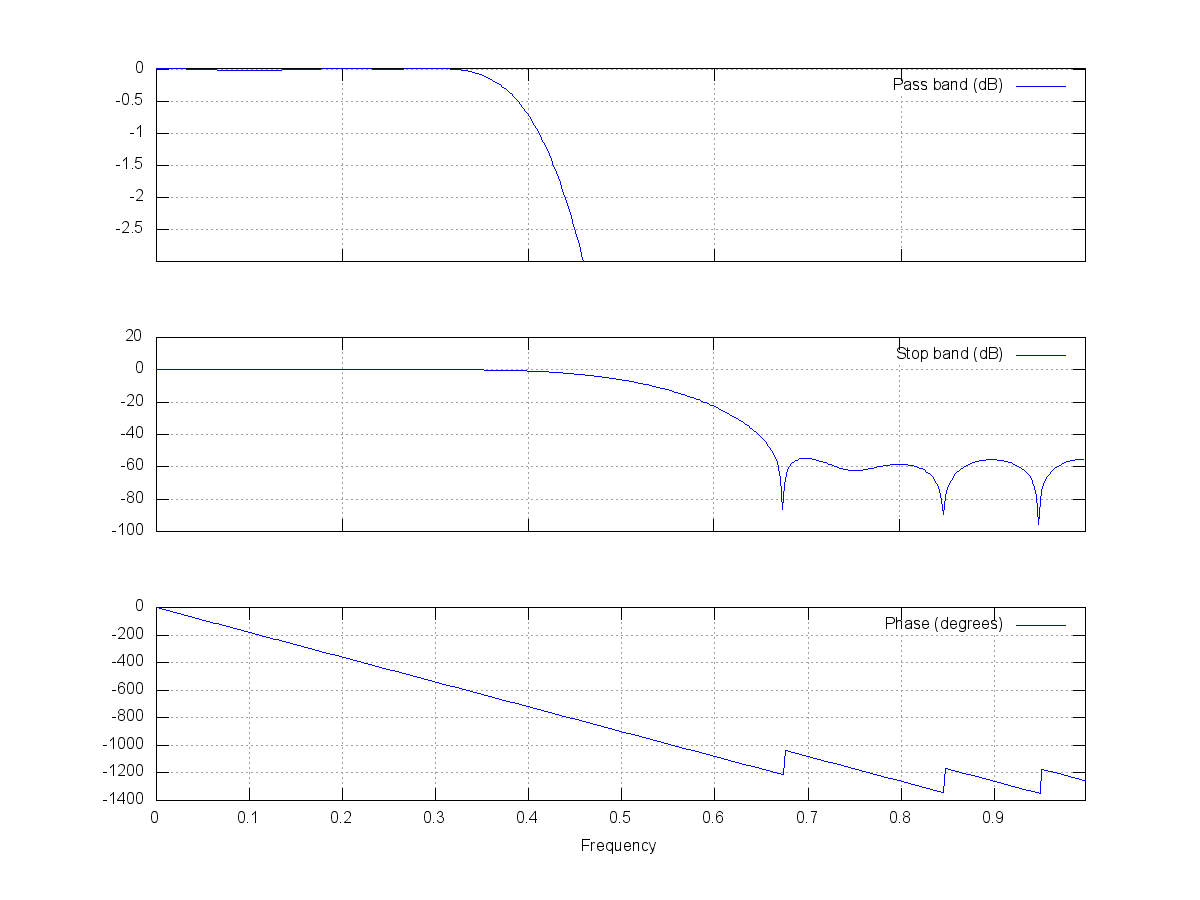
\includegraphics[scale=.5]{out/fig3.png}
	      \caption{\label{fig3}  Rząd filtru: 20}
	    \end{center}
	  \end{figure}
	\end{landscape}
	
	\begin{landscape}
	  \begin{figure}[htbp]
	    \begin{center}
	      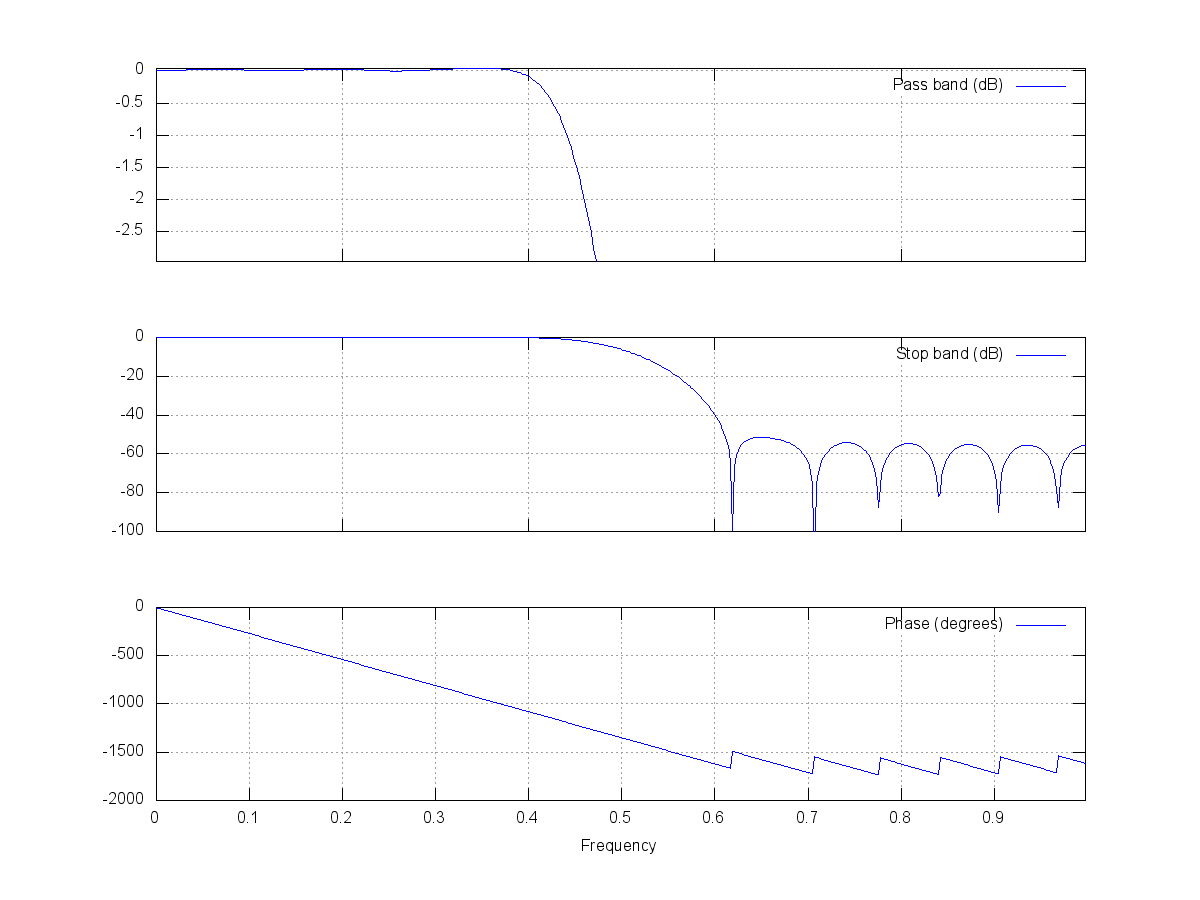
\includegraphics[scale=.5]{out/fig4.png}
	      \caption{\label{fig4} Rzad filtru 30}
	    \end{center}
	  \end{figure}
	\end{landscape}
	
	\begin{landscape}
	  \begin{figure}[htbp]
	    \begin{center}
	      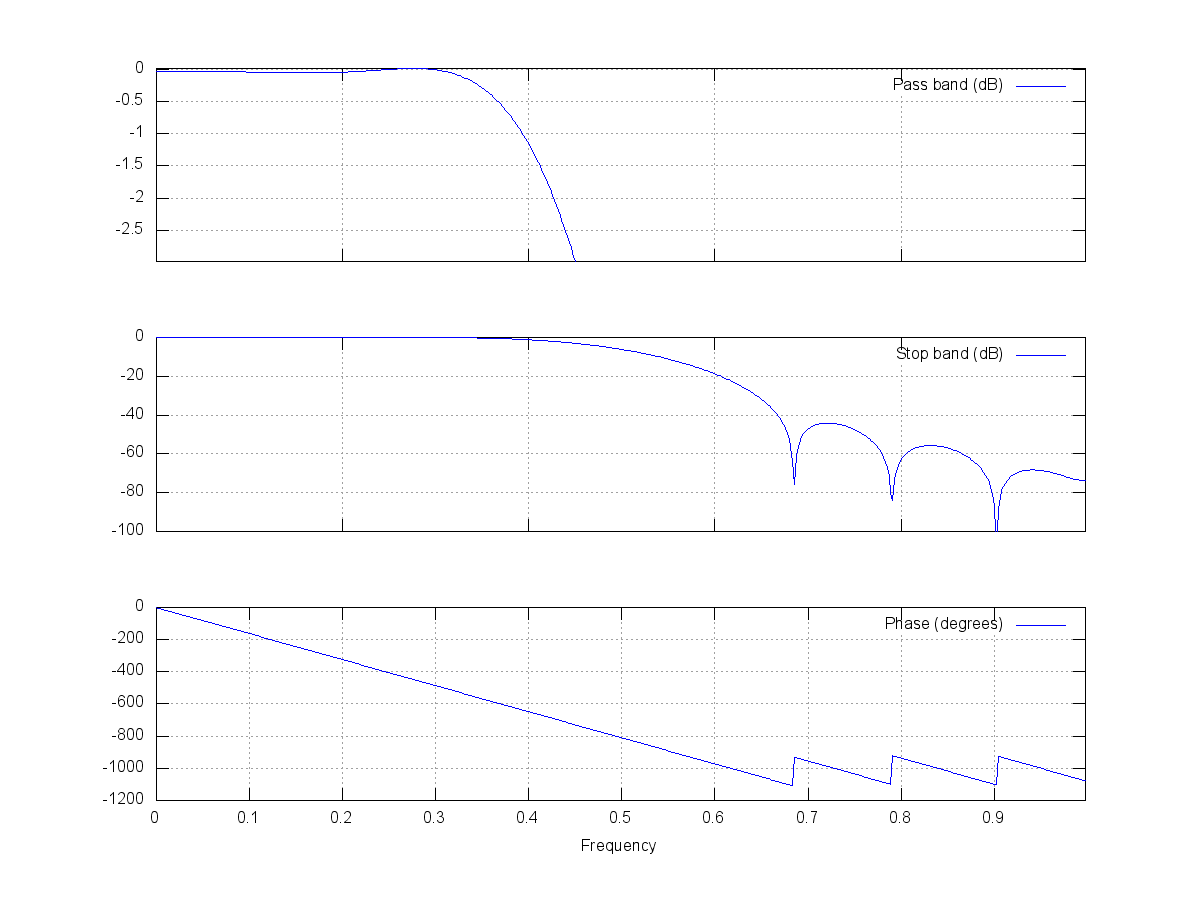
\includegraphics[scale=.5]{out/fig5.png}
	      \caption{\label{fig5} Okno $hanning$}
	    \end{center}
	  \end{figure}
	\end{landscape}
	
	\begin{landscape}
	  \begin{figure}[htbp]
	    \begin{center}
	      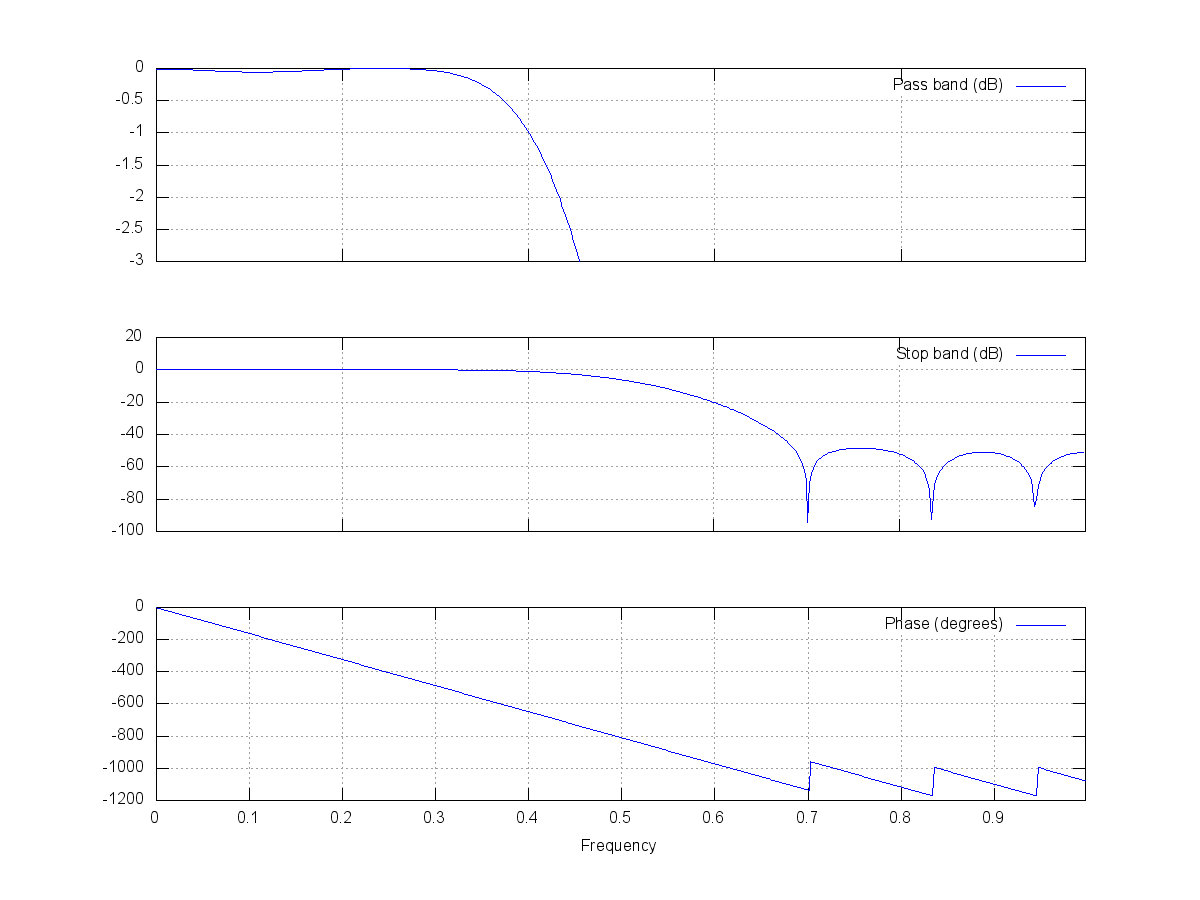
\includegraphics[scale=.5]{out/fig6.png}
	      \caption{\label{fig6} Okno $hamming$}
	    \end{center}
	  \end{figure}
	\end{landscape}
	
	\begin{landscape}
	  \begin{figure}[htbp]
	    \begin{center}
	      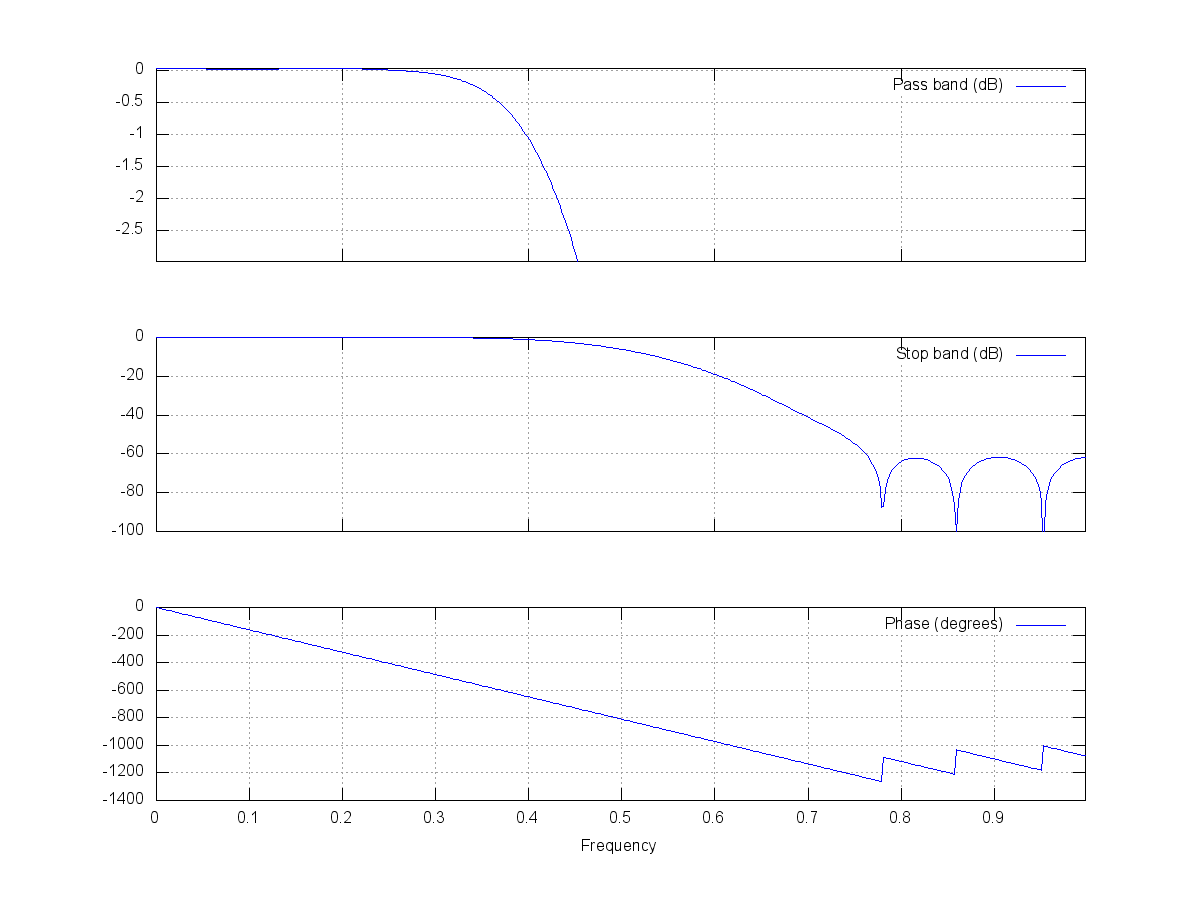
\includegraphics[scale=.5]{out/fig7.png}
	      \caption{\label{fig7} Okno $gausswin$}
	    \end{center}
	  \end{figure}
	\end{landscape}
	
	\begin{landscape}
	  \begin{figure}[htbp]
	    \begin{center}
	      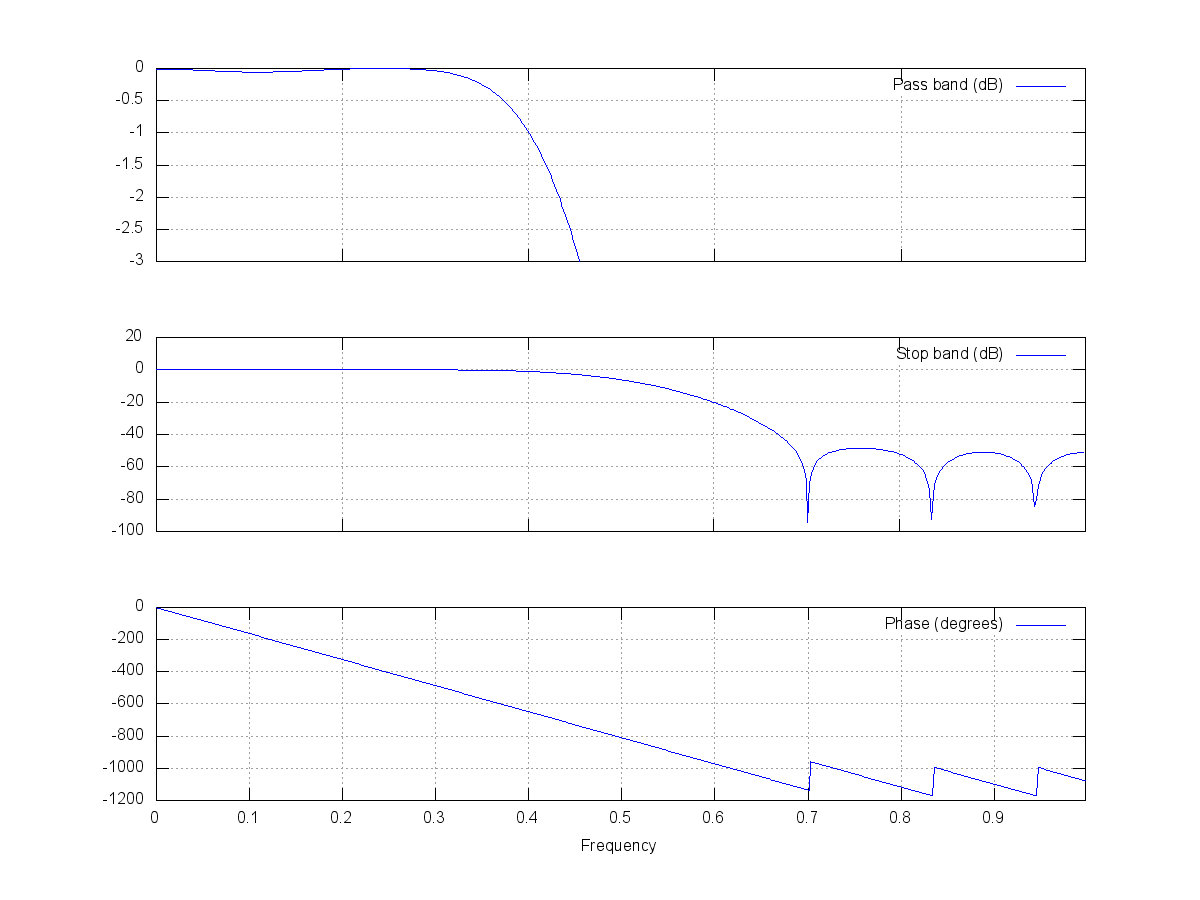
\includegraphics[scale=.5]{out/fig6.png}
	      \caption{\label{fig6} Okno $bartlett$}
	    \end{center}
	  \end{figure}
	\end{landscape}
	
	\begin{landscape}
	  \begin{figure}[htbp]
	    \begin{center}
	      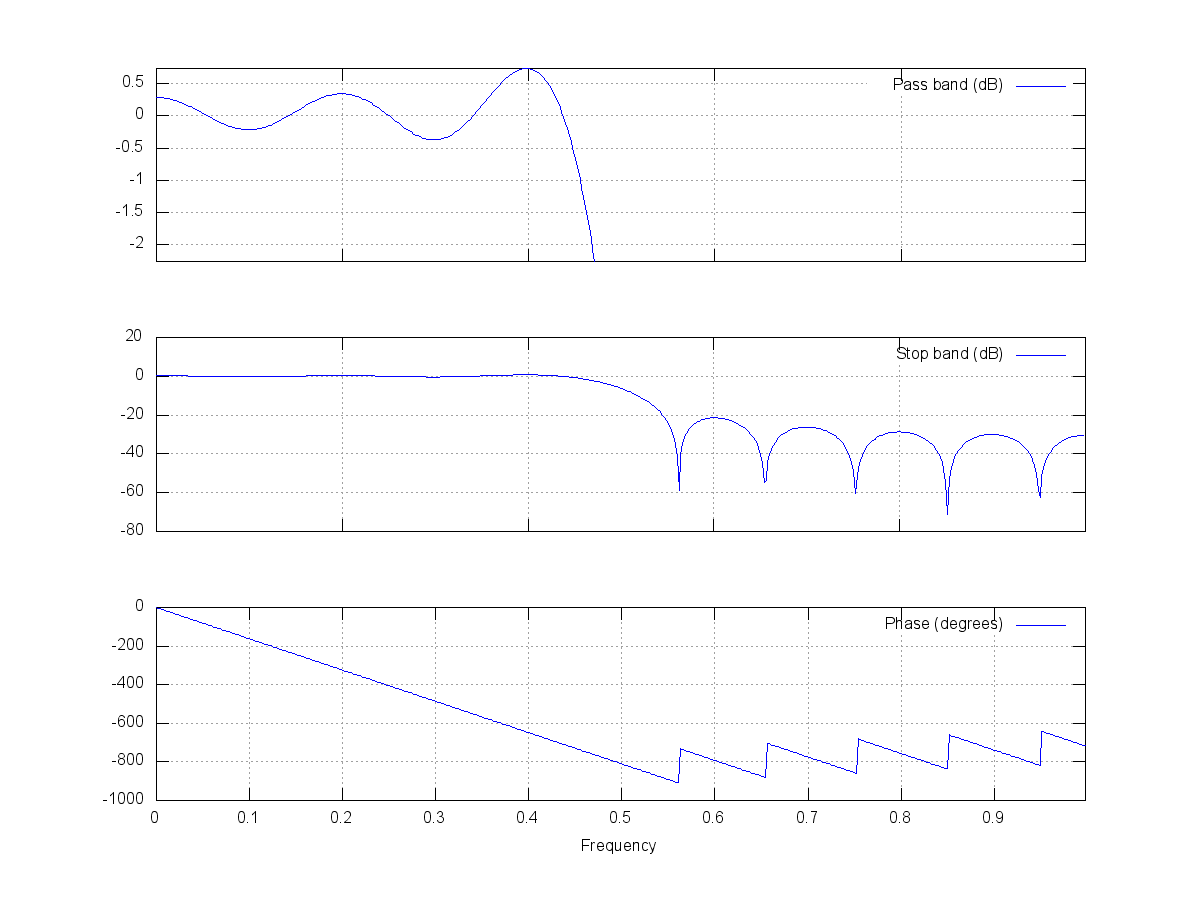
\includegraphics[scale=.5]{out/fig9.png}
	      \caption{\label{fig9} Okno $kaiser$}
	    \end{center}
	  \end{figure}
	\end{landscape}
	

\end{document}